\documentclass[12pt, twoside]{book}



\usepackage[a4paper,top=2.5cm,bottom=2.5cm,left=3.5cm,right=2cm]{geometry}
\usepackage[utf8]{inputenc}
\usepackage[T1]{fontenc}
\usepackage[slovak]{babel}


\linespread{1.25} 

% balicek na vkladanie zdrojoveho kodu
\usepackage{listings}
% ukazky kodu su cislovane ako Listing 1,2,...
% tu je Listing zmenene na Algoritmus 1,2,...
\renewcommand{\lstlistingname}{Algoritmus}
% nastavenia balicka listings
% mozete pridat aj language=...
% na nastavenie najcastejsie pouzivaneho prog. jazyka
% takisto sa da zapnut cislovanie riadkov
\lstset{frame=lines}


\usepackage{graphicx}
\usepackage{pdfpages}
\usepackage{url}
\usepackage[hidelinks,breaklinks]{hyperref}

% --- Definicia zakladnych pojmov

\def\mfrok{2023}
\def\mfnazov{Štatistická analýza multivariačných údajov: Prieskum spokojnosti študentov slovenských vysokých škôl}
\def\mftyp{Bakalárska práca}
\def\mfautor{Roman Hudec}
\def\mfskolitel{prof. Mgr. Martin Kanovský, PhD. }
\def\mfmiesto{Bratislava, \mfrok}

\def\mfodbor{ Informatika a Matematika } 
\def\program{ Dátová veda }

% Ak je školiteľ z FMFI, uvádzate katedru školiteľa, zrejme by mala byť aj na zadaní z AIS2
% Ak máte externého školiteľa, uvádzajte Katedru informatiky 
\def\mfpracovisko{ Katedra informatiky }

\begin{document}     
\frontmatter
\pagestyle{empty}


% --- Obalka ------
\begin{center}
\sc\large
Univerzita Komenského v Bratislave\\
Fakulta matematiky, fyziky a informatiky

\vfill

{\LARGE\mfnazov}\\
\mftyp
\end{center}

\vfill

{\sc\large 
\noindent \mfrok\\
\mfautor
}

\cleardoublepage
% --- koniec obalky ----

% --- Titulný list
\noindent

\begin{center}
\sc  
\large
Univerzita Komenského v Bratislave\\
Fakulta matematiky, fyziky a informatiky

\vfill

{\LARGE\mfnazov}\\
\mftyp
\end{center}

\vfill

\noindent
\begin{tabular}{ll}
Študijný program: & \program \\
Študijný odbor: & \mfodbor \\
Školiace pracovisko: & \mfpracovisko \\
Školiteľ: & \mfskolitel \\
\end{tabular}

\vfill


\noindent \mfmiesto\\
\mfautor

\cleardoublepage
% --- Koniec titulnej strany



% --- Zadanie z AIS
\newpage 
\setcounter{page}{2}
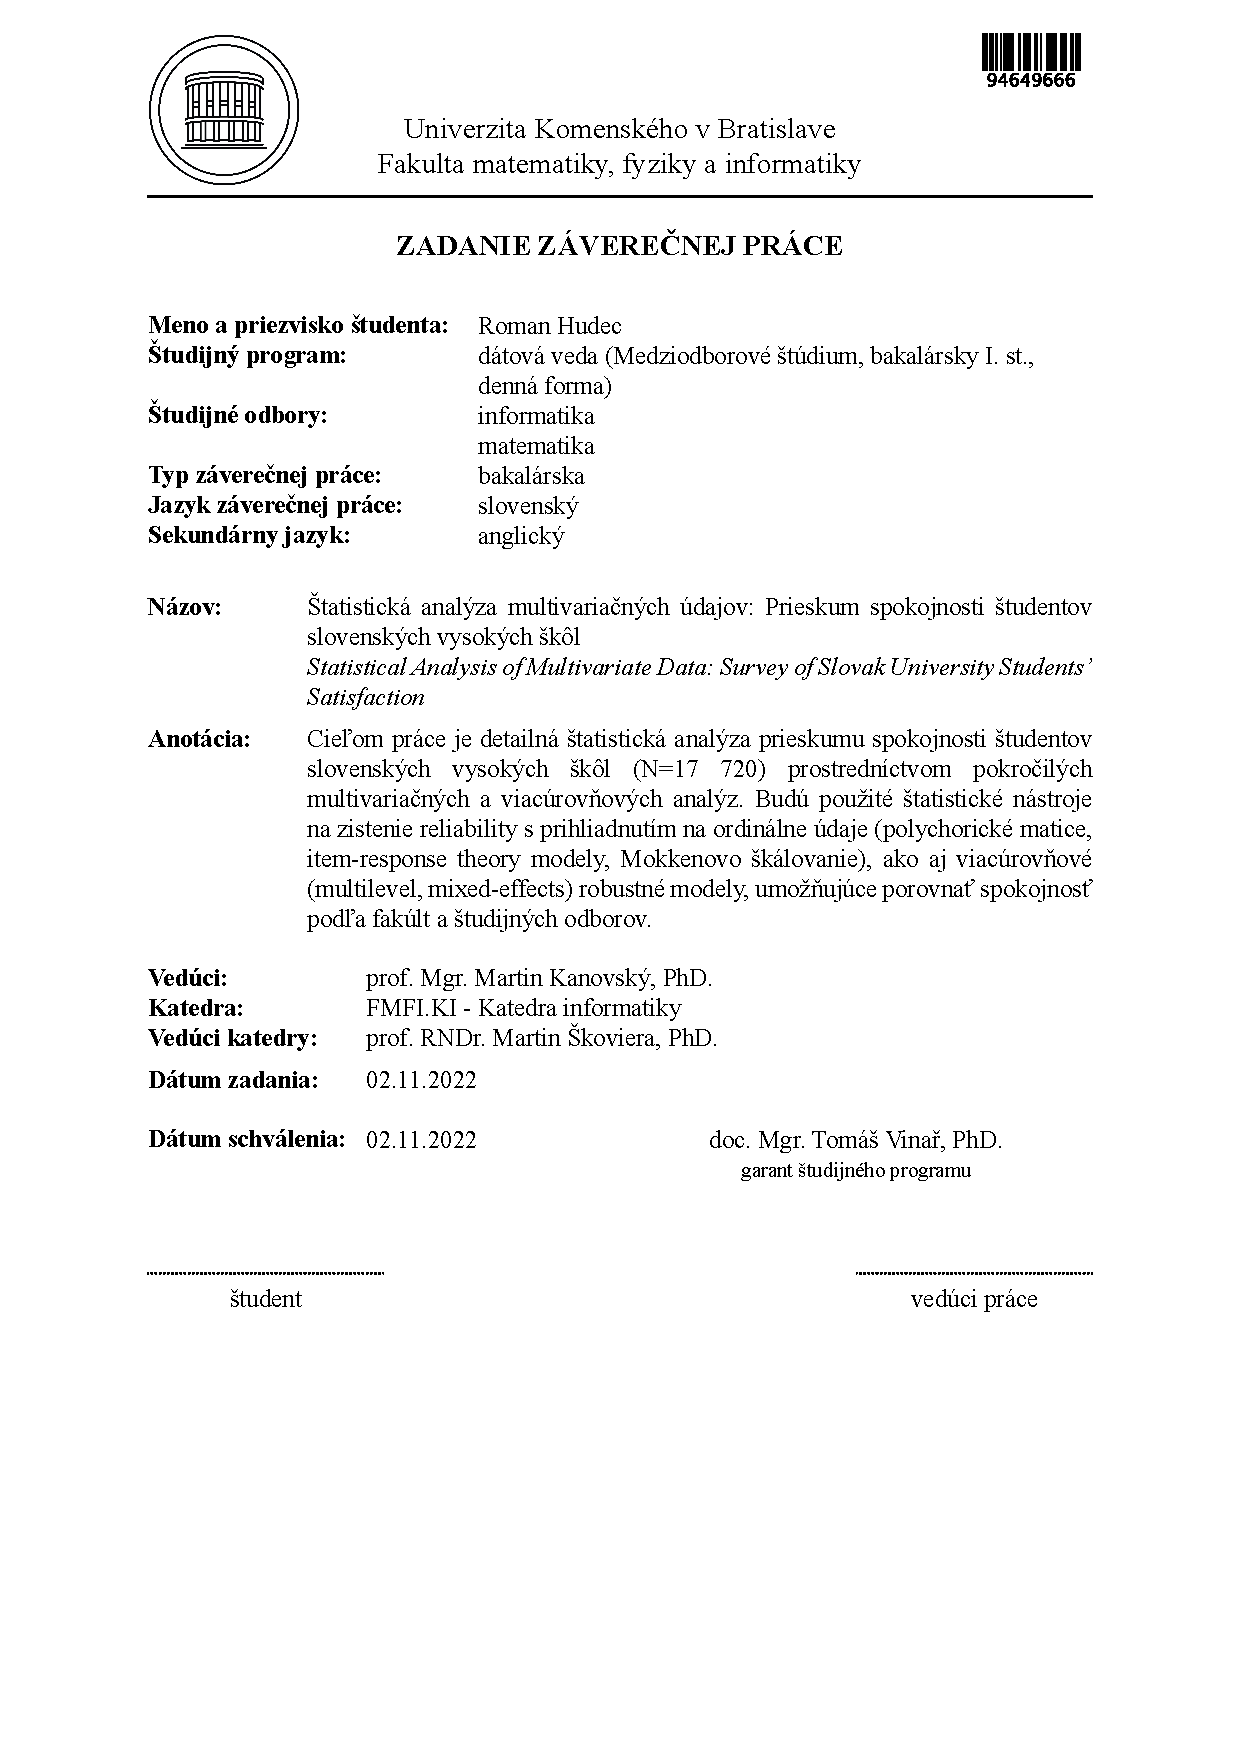
\includepdf{images/zadanie.pdf}

% --- Koniec zadania



%   Poďakovanie - nepovinné

\newpage 
\pagestyle{plain}
~

\vfill
{\bf Poďakovanie:}

% --- Koniec poďakovania

% -------------------
%   Abstrakt - Slovensky
% -------------------
\newpage 
\section*{Abstrakt}


\paragraph*{Kľúčové slová:}



% --- Abstrakt - Anglicky 
\newpage 
\section*{Abstract}


\paragraph*{Keywords:} 

% --- Koniec Abstrakt - Anglicky


% --- Predhovor - v informatike sa zvacsa nepouziva

%\newpage 
%
%\chapter*{Predhovor}
%
%Predhovor je všeobecná informácia o práci, obsahuje hlavnú charakteristiku práce 
%a okolnosti jej vzniku. Autor zdôvodní výber témy, stručne informuje o cieľoch 
%a význame práce, spomenie domáci a zahraničný kontext, komu je práca určená, 
%použité metódy, stav poznania; autor stručne charakterizuje svoj prístup a svoje 
%hľadisko. 
%
% --- Koniec Predhovor



% --- Obsah
\newpage 

\tableofcontents
% ---  Koniec Obsahu


% --- Zoznamy tabuliek, obrázkov - nepovinne

\newpage 

%\listoffigures
%\listoftables

% ---  Koniec Zoznamov

\mainmatter
\pagestyle{headings}

%zakomentovať ku koncu

\input uvod.tex 

\input ciel.tex

\input metodika.tex

\input vysledky.tex

\input zaver.tex

% --- Bibliografia
\newpage	

\backmatter

\thispagestyle{empty}
\clearpage

\bibliographystyle{plain}
\bibliography{literatura} 

%---koniec Referencii

%--- Prilohy---

%Nepovinná časť prílohy obsahuje materiály, ktoré neboli zaradené priamo  do textu. Každá príloha sa začína na novej strane.
%Zoznam príloh je súčasťou obsahu.
%
%\input appendixA.tex

%\input appendixB.tex

\end{document}






